\documentclass[12pt]{report}
\usepackage[utf8]{inputenc}
\usepackage[russian]{babel}
%\usepackage[14pt]{extsizes}
\usepackage{listings}
\usepackage{graphicx}
\usepackage{amsmath,amsfonts,amssymb,amsthm,mathtools} 
\usepackage{pgfplots}
\usepackage{filecontents}
\usepackage{float}
\usepackage{comment}
\usepackage{indentfirst}
\usepackage{eucal}
\usepackage{enumitem}
%s\documentclass[openany]{book}
\frenchspacing

\usepackage{indentfirst} % Красная строка

\usetikzlibrary{datavisualization}
\usetikzlibrary{datavisualization.formats.functions}

\usepackage{amsmath}


% Для листинга кода:
\lstset{ %
	language=c,                 % выбор языка для подсветки (здесь это С)
	basicstyle=\small\sffamily, % размер и начертание шрифта для подсветки кода
	numbers=left,               % где поставить нумерацию строк (слева\справа)
	numberstyle=\tiny,           % размер шрифта для номеров строк
	stepnumber=1,                   % размер шага между двумя номерами строк
	numbersep=5pt,                % как далеко отстоят номера строк от подсвечиваемого кода
	showspaces=false,            % показывать или нет пробелы специальными отступами
	showstringspaces=false,      % показывать или нет пробелы в строках
	showtabs=false,             % показывать или нет табуляцию в строках
	frame=single,              % рисовать рамку вокруг кода
	tabsize=2,                 % размер табуляции по умолчанию равен 2 пробелам
	captionpos=t,              % позиция заголовка вверху [t] или внизу [b] 
	breaklines=true,           % автоматически переносить строки (да\нет)
	breakatwhitespace=false, % переносить строки только если есть пробел
	escapeinside={\#*}{*)}   % если нужно добавить комментарии в коде
}


\usepackage[left=2cm,right=2cm, top=2cm,bottom=2cm,bindingoffset=0cm]{geometry}
% Для измененных титулов глав:
\usepackage{titlesec, blindtext, color} % подключаем нужные пакеты
\definecolor{gray75}{gray}{0.75} % определяем цвет
\newcommand{\hsp}{\hspace{20pt}} % длина линии в 20pt
% titleformat определяет стиль
\titleformat{\chapter}[hang]{\Huge\bfseries}{\thechapter\hsp\textcolor{gray75}{|}\hsp}{0pt}{\Huge\bfseries}


% plot
\usepackage{pgfplots}
\usepackage{filecontents}
\usetikzlibrary{datavisualization}
\usetikzlibrary{datavisualization.formats.functions}

\begin{document}
	%\def\chaptername{} % убирает "Глава"
	\thispagestyle{empty}
	\begin{titlepage}
		\noindent \begin{minipage}{0.15\textwidth}
			
\includegraphics[width=\linewidth]{img/b_logo}
		\end{minipage}
		\noindent\begin{minipage}{0.9\textwidth}\centering
			\textbf{Министерство науки и высшего образования Российской Федерации}\\
			\textbf{Федеральное государственное бюджетное образовательное учреждение высшего образования}\\
			\textbf{~~~«Московский государственный технический университет имени Н.Э.~Баумана}\\
			\textbf{(национальный исследовательский университет)»}\\
			\textbf{(МГТУ им. Н.Э.~Баумана)}
		\end{minipage}
		
		\noindent\rule{18cm}{3pt}
		\newline\newline
		\noindent ФАКУЛЬТЕТ $\underline{\text{«Информатика и системы управления»}}$ \newline\newline
		\noindent КАФЕДРА $\underline{\text{«Программное обеспечение ЭВМ и информационные технологии»}}$\newline\newline\newline\newline\newline
		
		\begin{center}
			\noindent\begin{minipage}{1.1\textwidth}\centering
				\Large\textbf{  Отчет по лабораторной работе №6}\newline
				\textbf{по дисциплине <<Операционные системы>>}\newline\newline\newline
			\end{minipage}
		\end{center}
		
		\noindent\textbf{Тема} $\underline{\text{Системный вызов \texttt{open}~~~~~}}$\newline\newline
		\noindent\textbf{Студент} $\underline{\text{Романов А.В.~~~~~~~~~~~~~}}$\newline\newline
		\noindent\textbf{Группа} $\underline{\text{ИУ7-63Б~~~~~~~~~~~~~~~~~~~~~}}$\newline\newline
		\noindent\textbf{Оценка (баллы)} $\underline{\text{~~~~~~~~~~~~~~~~~~~~}}$\newline\newline
		\noindent\textbf{Преподаватель} $\underline{\text{Рязанова Н. Ю.}}$\newline\newline\newline
		
		\begin{center}
			\vfill
			Москва~---~\the\year
			~г.
		\end{center}
	\end{titlepage}


\chapter{Используемые структуры}

\begin{lstlisting}[language=c, label=lst:filename, caption=Листинг структуры filename]
struct filename {
	const char		*name;	/* pointer to actual string */
	const __user char	*uptr;	/* original userland pointer */
	int			refcnt;
	struct audit_names	*aname;
	const char		iname[];
};
\end{lstlisting}

\begin{lstlisting}[language=c, label=lst:open_flags, caption=Листинг структуры open\_flags]
struct open_flags {
	int open_flag;
	umode_t mode;
	int acc_mode;
	int intent;
	int lookup_flags;
};
\end{lstlisting}

\begin{lstlisting}[language=c, label=lst:nameidata, caption=Листинг структуры nameidata]

#define EMBEDDED_LEVELS 2
	struct nameidata {
	struct path	path;
	struct qstr	last;
	struct path	root;
	struct inode	*inode; /* path.dentry.d_inode */
	unsigned int	flags;
	unsigned	seq, m_seq, r_seq;
	int		last_type;
	unsigned	depth;
	int		total_link_count;
	struct saved {
	struct path link;
		struct delayed_call done;
		const char *name;
		unsigned seq;
	} *stack, internal[EMBEDDED_LEVELS];
	struct filename	*name;
	struct nameidata *saved;
	unsigned	root_seq;
	int		dfd;
	kuid_t		dir_uid;
	umode_t		dir_mode;
} __randomize_layout;
\end{lstlisting}

\chapter{Схемы алгоритмов}

\begin{figure}[H]
	\centering
	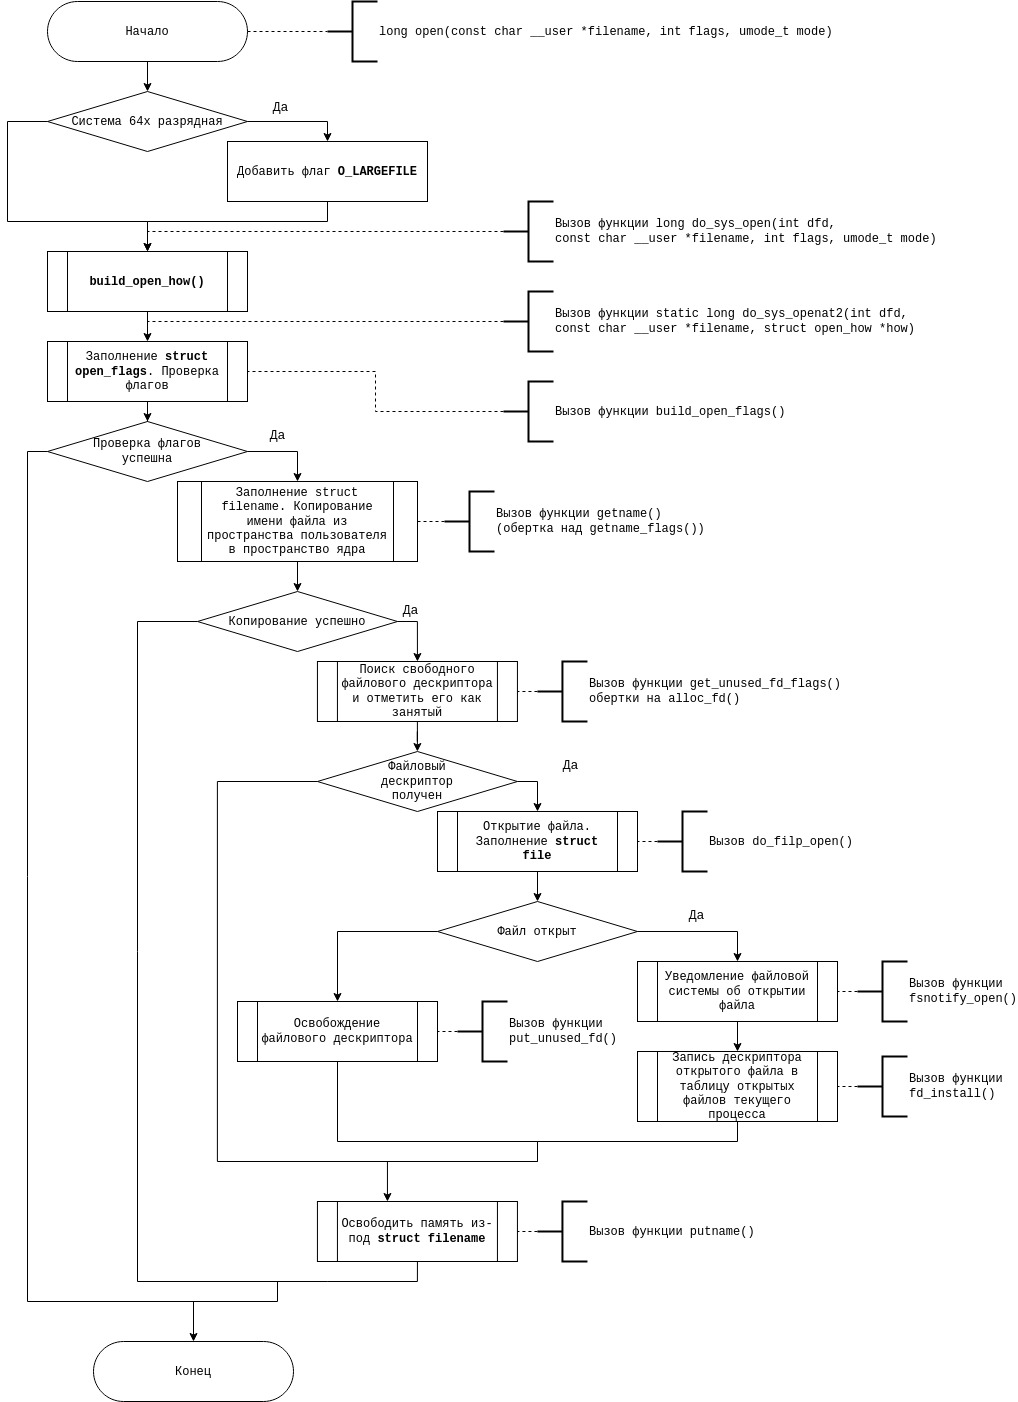
\includegraphics[scale=0.41]{img/open.jpg}
	\label{fig:open}
\end{figure}

\section{Схема работы алгоритма функции $\texttt{build\_open\_flags}$}

\begin{figure}[H]
	\centering
	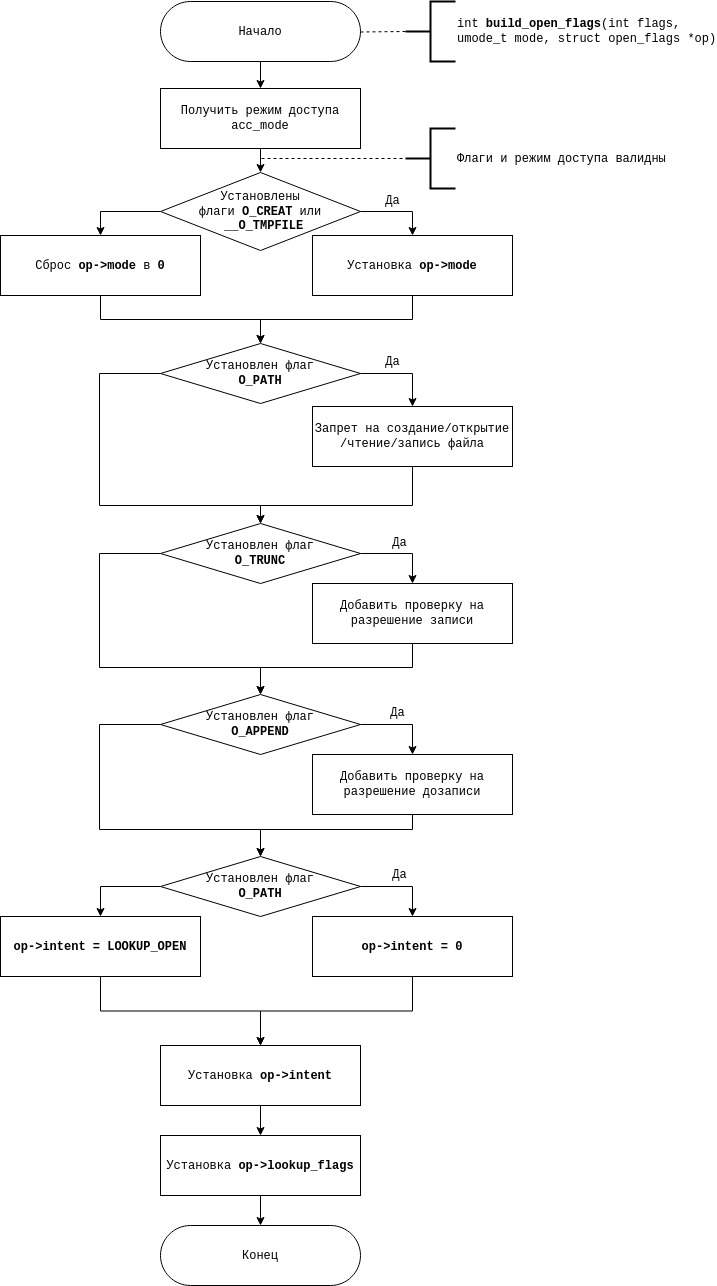
\includegraphics[scale=0.5]{img/build_open_flags.jpg}
	%\caption{Схема структур программы №1}
	\label{fig:open_open_flags}
\end{figure}

\section{Схема работы алгоритма функции $\texttt{getname\_flags}$}

\begin{figure}[H]
	\centering
	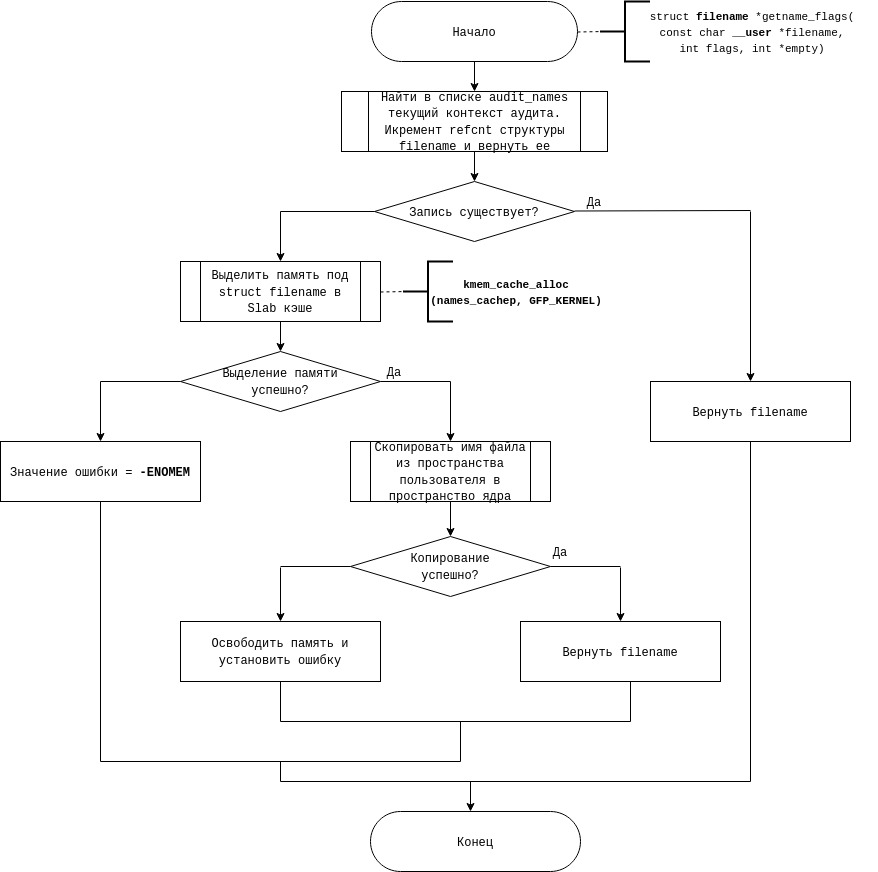
\includegraphics[scale=0.4]{img/getname_flags.jpg}
	%\caption{Схема структур программы №1}
	\label{fig:get_name_flags}
\end{figure}

\section{Схема работы алгоритма функции $\texttt{alloc\_fd}$}

\begin{figure}[H]
	\centering
	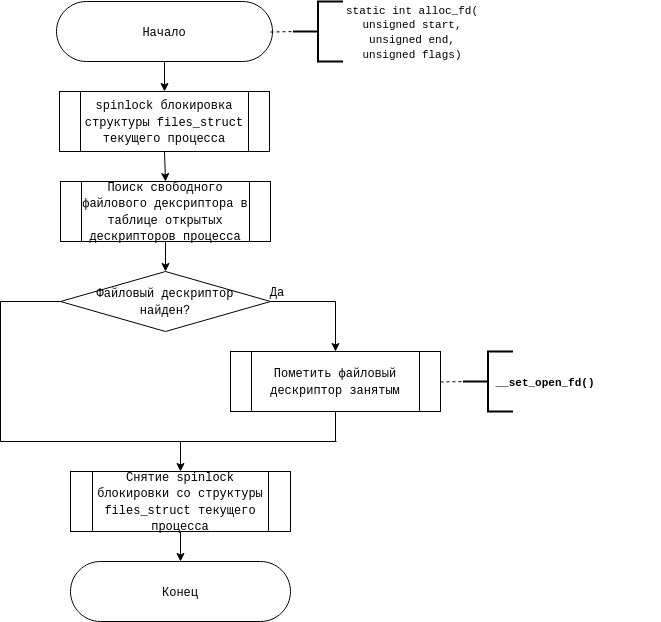
\includegraphics[scale=0.35]{img/alloc_fd.jpg}
	%\caption{Схема структур программы №1}
	\label{fig:alloc_fd}
\end{figure}

\section{Схема работы алгоритма функции $\texttt{path\_openat}$}

\begin{figure}[H]
	\centering
	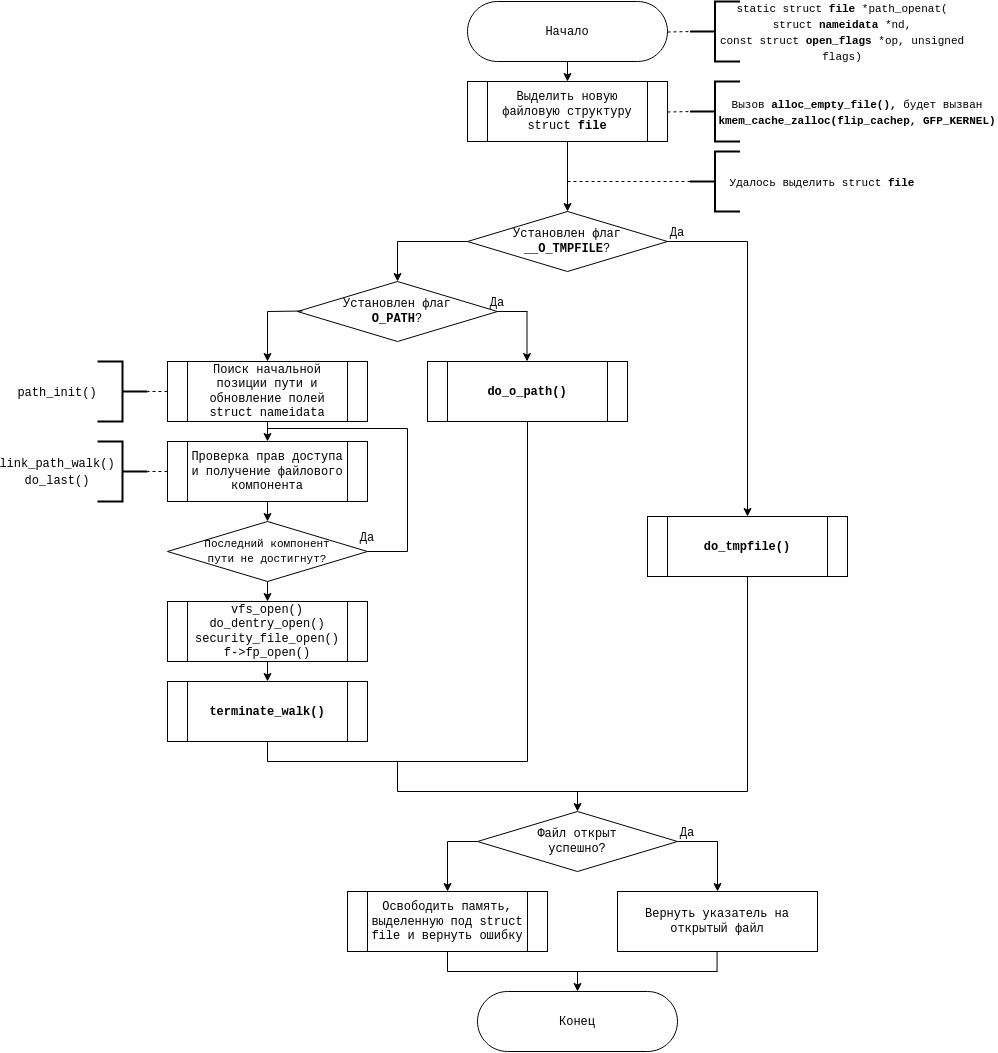
\includegraphics[scale=0.54]{img/path_openat.jpg}
	%\caption{Схема структур программы №1}
	\label{fig:path_openat}
\end{figure}

\section{Схема работы алгоритма функции $\texttt{do\_last}$}

\begin{figure}[H]
	\centering
	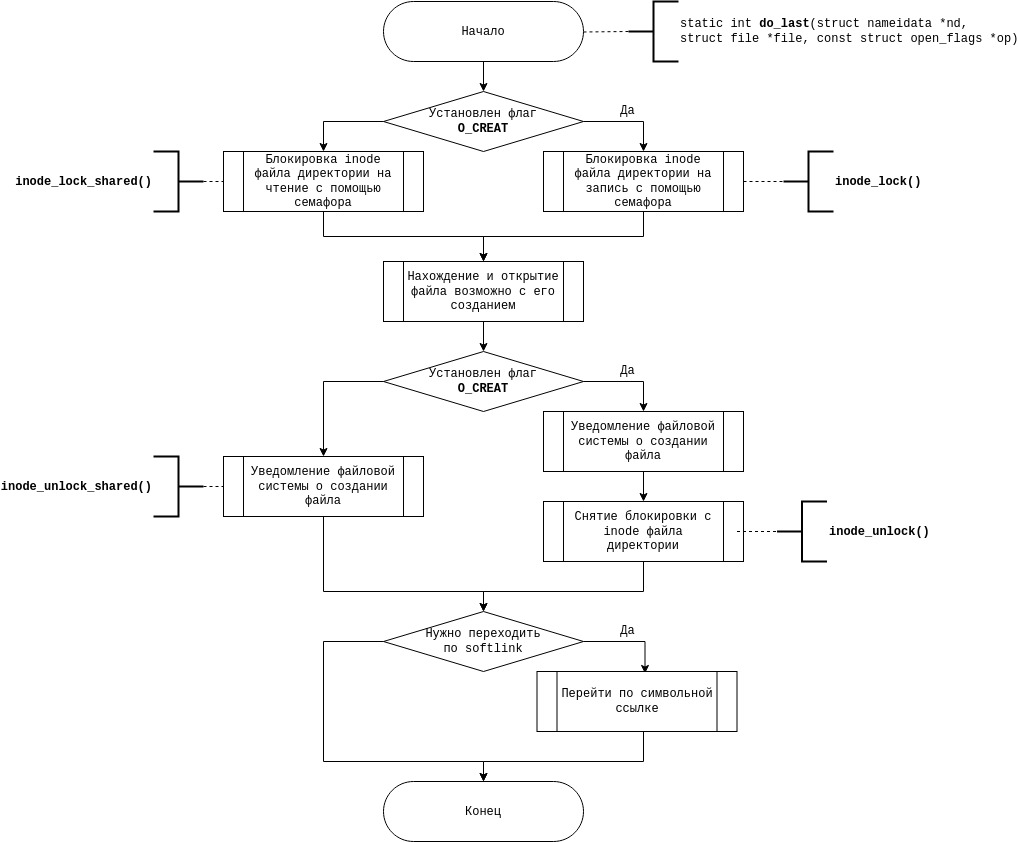
\includegraphics[scale=0.52]{img/do_last.jpg}
	%\caption{Схема структур программы №1}
	\label{fig:do_last}
\end{figure}

\section{Схема работы алгоритма функции $\texttt{lookup\_open}$}

\begin{figure}[H]
	\centering
	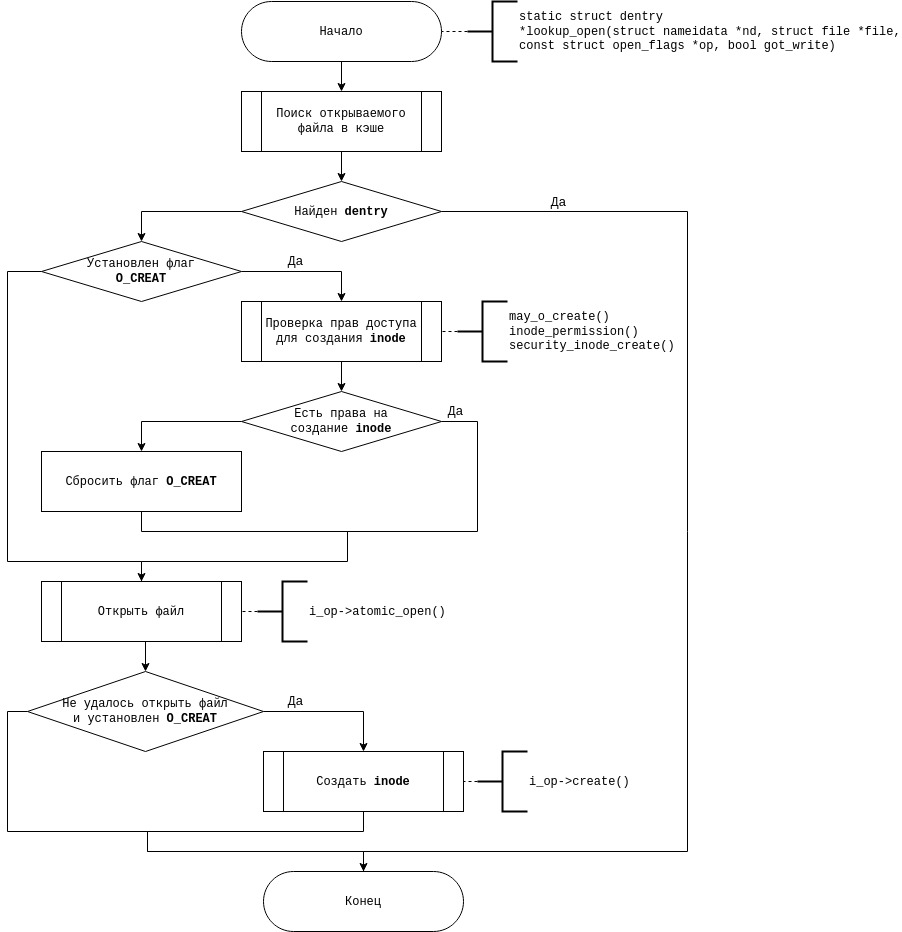
\includegraphics[scale=0.6]{img/lookup_open.jpg}
	%\caption{Схема структур программы №1}
	\label{fig:lookup_open}
\end{figure}

\bibliographystyle{utf8gost705u}  % стилевой файл для оформления по ГОСТу
\bibliography{51-biblio}          % имя библиографической базы (bib-файла)
	
\end{document}
